\documentclass[a4paper, 10pt]{article}
\usepackage[margin=0.5in]{geometry}

\usepackage{blindtext}
\usepackage{multicol}
\usepackage{booktabs}
\usepackage{amsmath}
\usepackage{mathtools}
\usepackage{float}
\usepackage{graphicx}
\usepackage{enumitem}
\usepackage{hyperref}
\usepackage{comment}

\graphicspath{ {../outputs/}{../data/} }


\setlength{\columnsep}{1cm}
\title{ENPM 673: Perception for Autonomous Robots - Project 1}
\author{Aswath Muthuselvam \\ aswath@umd.edu}
\date{26th Feb 2022}

\begin{document}
	\maketitle
	\newlist{contract}{enumerate}{10}
	\setlist[contract]{label*=\arabic*.}
	\setlistdepth{10} 
	
	\begin{multicols}{2}
		
		\section{Problem 1}
		\subsection{A) AR Code detection}
		
		A robot need to make sense of it's surroundings and able to localize itself with respect to it's surrounding environment. Problem 1a involves detection of AR Code. An AR Code is a marker that is used as an easy method of perceiving the environment by using simple algorithms rather than having to understand the entirety of the scene. 
		
		First, the sample video that is provided is relatively easier to process, with not many objects present in the scene. The sheet of paper that has AR Tag printed on it, can be located with performing image filtering techniques. The original image is taken and FFT(Fast Fourier Transform) is performed. Then, the zero of the frequency map is shifted to the center of the image. A circular Mask filled with value of zero is created, the values outside the circle is given as 1. The shifter frequency map is multiplied with the Mask to remove the low frequency components. The remaining high frequency values are converted back into an image by using Inverse-FFT Transform. Now the output of this operation provides us with only the edges of the paper and the AR Tag. 
		

		Finally, the AR Tag is warped to a square of size 128x128, the AR Tag is brought form the image space to a custom Top down - birds eye view.
		
		
		The detection of this tag involves multiple steps:
		\begin{enumerate}
			\item Pass the image through High Pass filter
			\begin{contract}
				\item Take Fourier Transform
				\item Frequency shift 
				\item Prepare a mask
				\item Apply the mask to filter the low frequency components.
			\end{contract}
			\item Apply inverse Fourier transform.
			\item Apply FFTShift
			\item Convert the image to binary and dilate the image. 
			\item Apply canny edge detection to make the the ARcode slightly round
			\item Use Blob detection to detect the near round arcode
			\item Take a template of the ARcode in top down view position
			\item Use SIFT feature matching on the blob and the template ARCode image to find the homography.
			\item Detect blob 
			
		\end{enumerate}
		
		\begin{figure}[H]
			\centering
			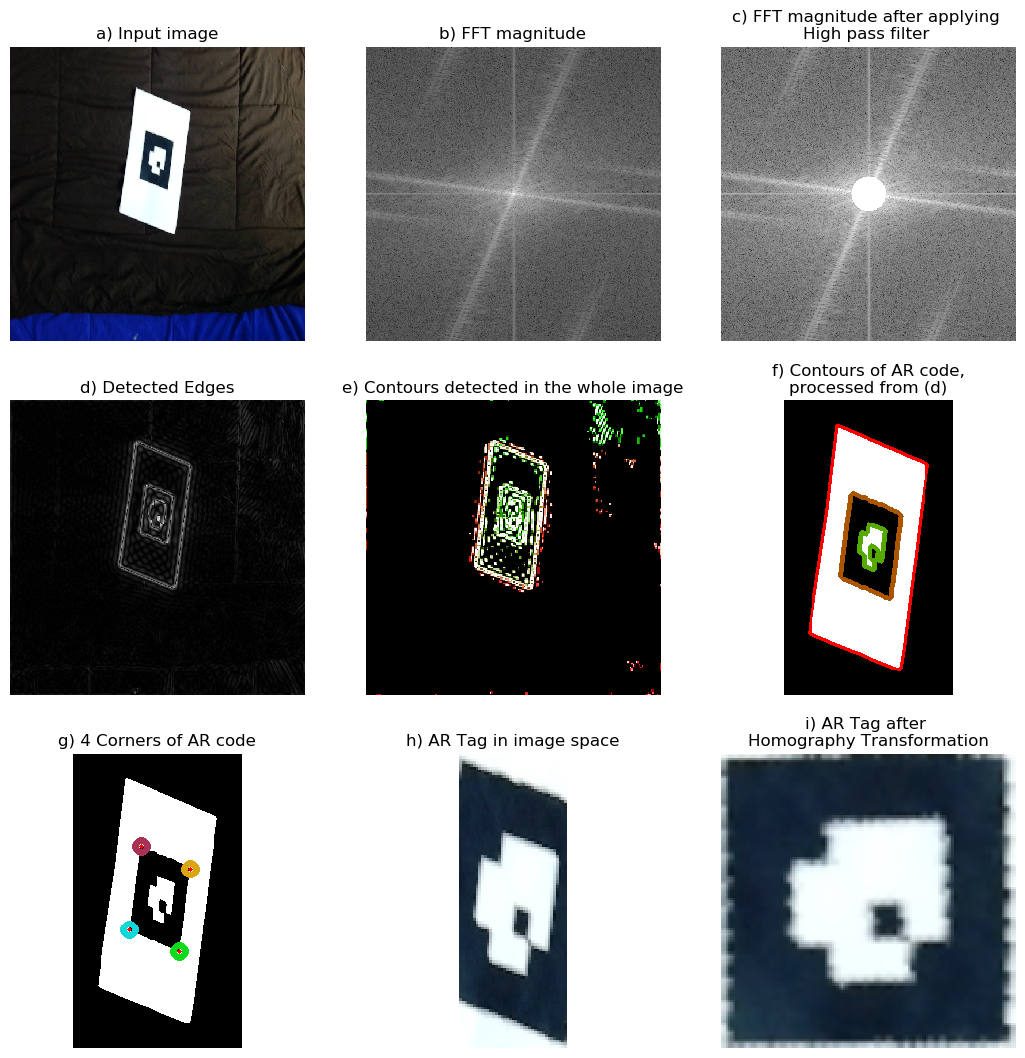
\includegraphics[width=\columnwidth]{/Q1/ARDetectionUsingFFt.png}
			\caption{AR Tag localization with FFT and Homography}
			\label{fig:FFT}
		\end{figure}
		
		\begin{comment}
		
		\begin{figure*}
		\centering
		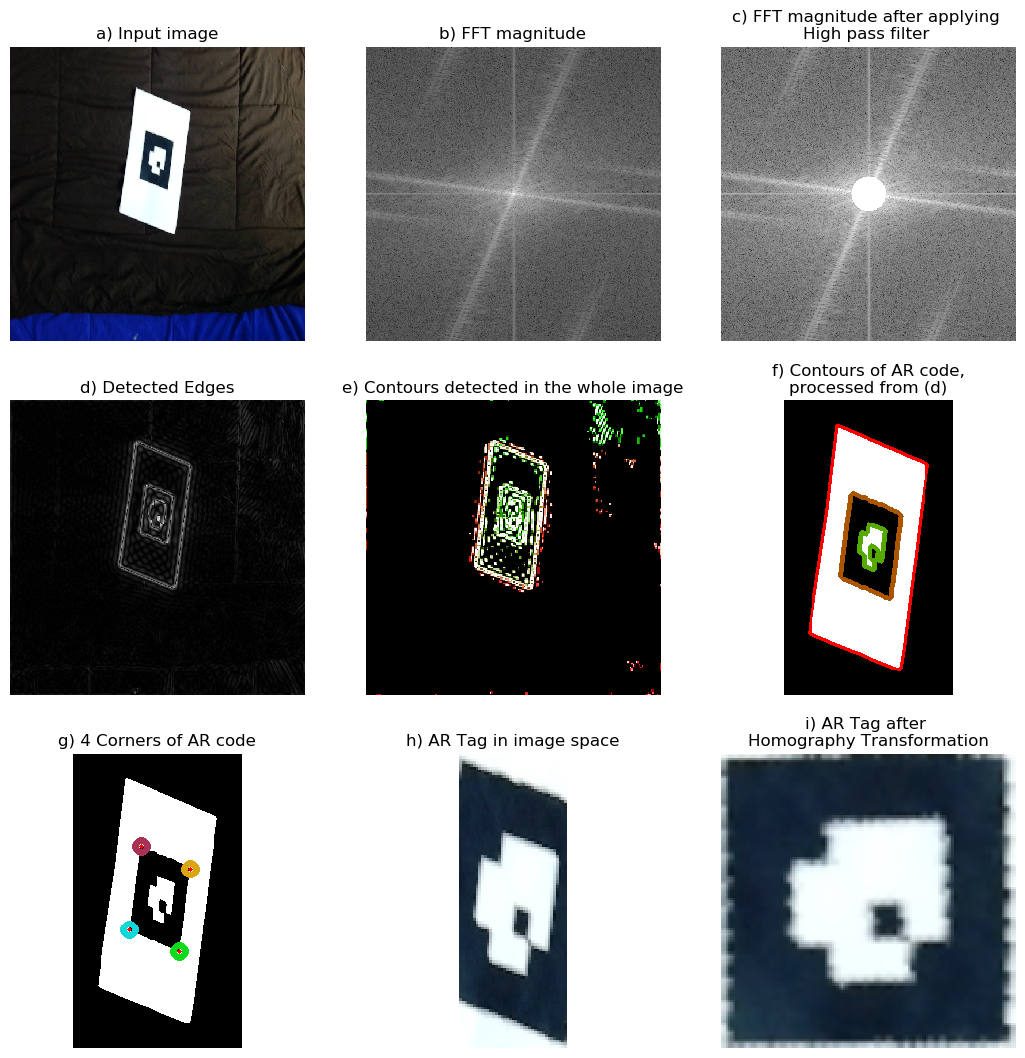
\includegraphics[width=0.75\textwidth]{/Q1/ARDetectionUsingFFt.png}
		\caption{Projecting the Testudo image on the ARTag}
		\label{fig:ARTa1g}
		\end{figure*}
		
		\end{comment}
		
		The homography transformation matrix is given by:
		\[
		\begin{bmatrix}
		x^{'} \\
		y^{'} \\
		w
		\end{bmatrix} =
		H\begin{bmatrix}
		x \\
		y \\
		1
		\end{bmatrix} = 
		\begin{bmatrix}
		h_{11} & h_{12} & h_{13}\\
		h_{21} & h_{22} & h_{23}\\
		h_{31} & h_{32} & h_{33}
		\end{bmatrix}
		\begin{bmatrix}
		x \\
		y \\
		1
		\end{bmatrix}
		\]
		
		\subsection{B) AR Code Decoding}
		An AR Code has two orthogonal protrusions on one corner. Using this feature, the orientation of the AR Code can be determined. The AR Code decoded by splitting the image into a 8x8 Grid and summing the pixel intensities in each grid.
		\begin{itemize}
		 \item The square image is converted to greyscale image and applied binary thresholding.
		\item The tag is split into 8x8 region, but our region of interest is only the middle 4x4 matrix which contains the id and the orientation of tag.
		\item Black is considered as 0 and white is considered as 1.
		\item In case of the white block being present at the bottom left corner, the orientation of the tag is bottom left.
		\item The innermost 2x2 matrix can be located and used for decoding based on least significant to the most significant bit. 
		\item The orientation of tag is used in superimposing the testudo image on the tag.
		\end{itemize}
		
		\begin{figure}[H]
			\centering
			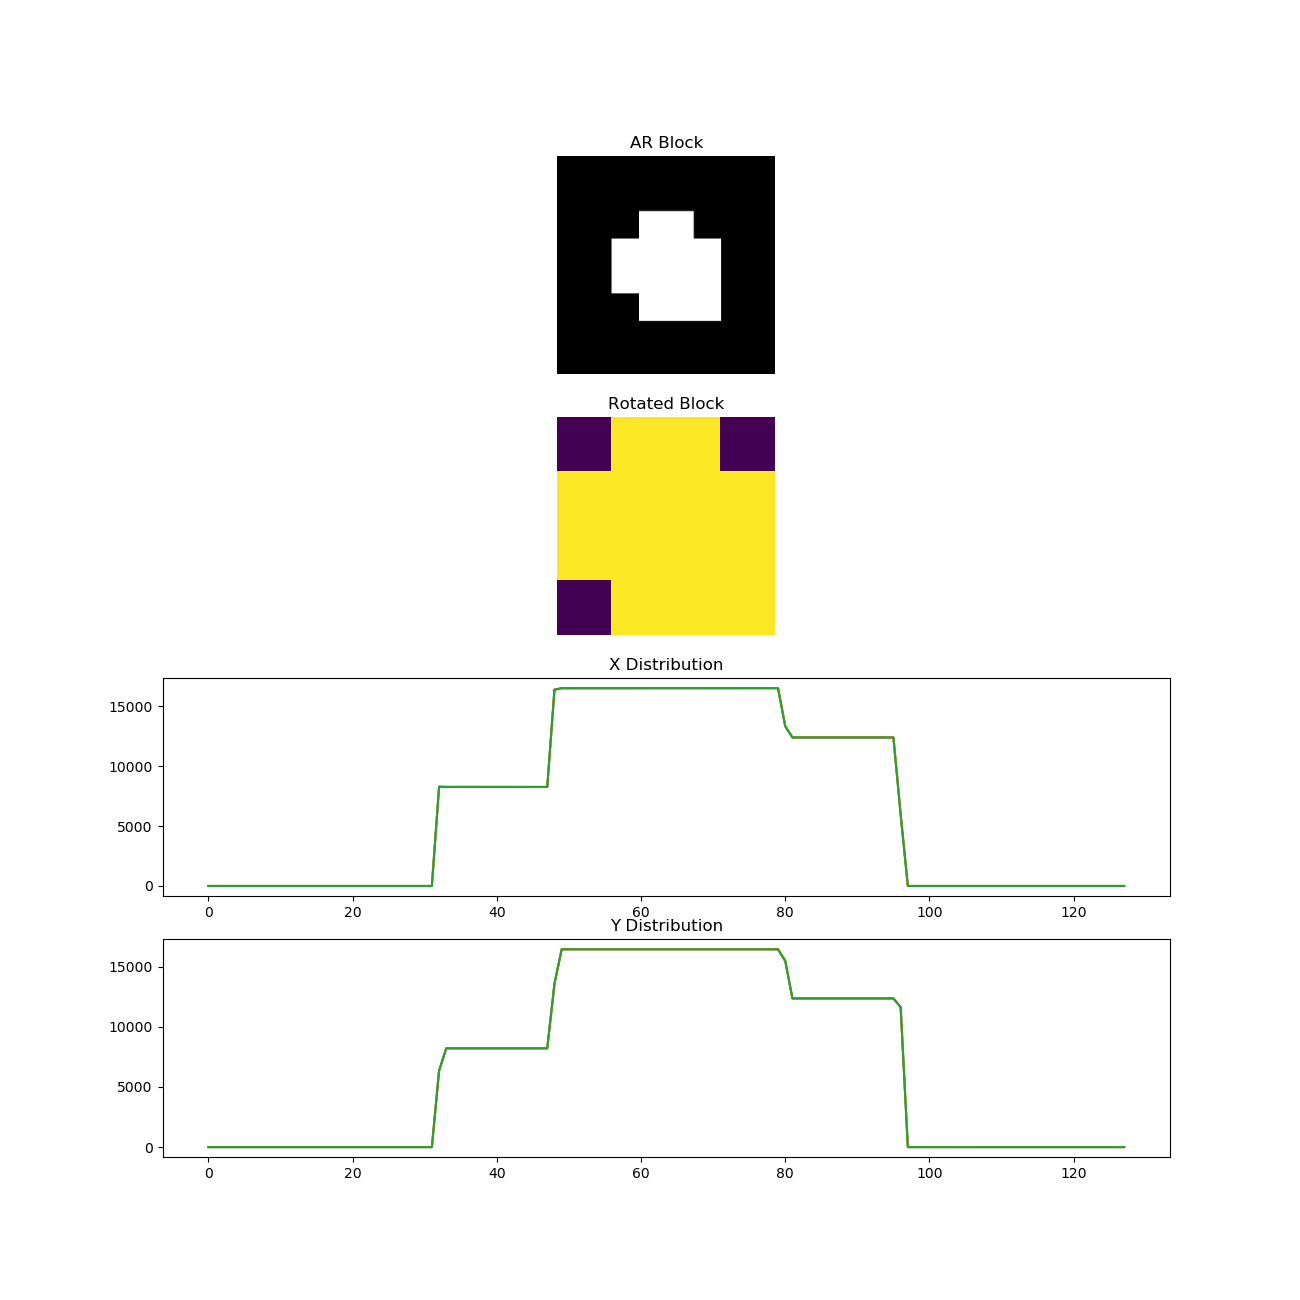
\includegraphics[width=\columnwidth]{/Q1/AR_Code_Decode.png}
			\caption{Decoding the AR Code}
			\label{fig:ARDecode}
		\end{figure}
		
		
		\section{Problem 2}
		
		Figure \ref{fig:ARTag} shows the projection of Testudo image on top of the AR Tag. 
		
		\begin{itemize}
		\item Firstly, the image is resized to the dimension of 200 x 200 to match the world coordinates.
		\item A “changeOrient” is defined to reorient the tag. The image, according to the orientation of the tag is rotated by using this function.
		\item After transformations and inverse homography, the tag in the image is warped to form a black background
		\item The function cv2.bitwise\_or is used to superimpose the testudo image on the AR tag.
		\end{itemize}
	
		\subsection{A) AR Testudo Projection}
		\begin{figure}[H]
			\centering
			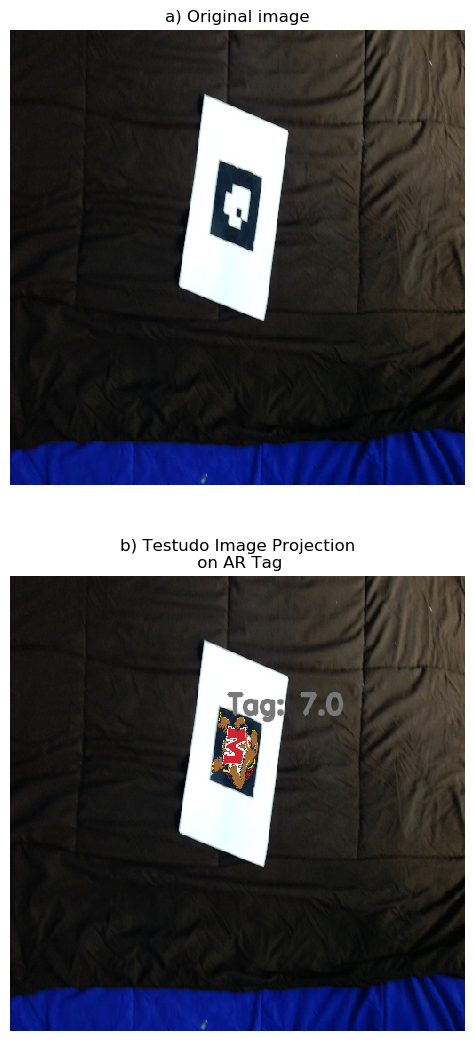
\includegraphics[width=\columnwidth]{/Q2/AR_Testudo_Projection.png}
			\caption{Projecting the Testudo image on the ARTag}
			\label{fig:ARTag}
		\end{figure}
		
		
		\subsection{B) AR Cube Projection}
		Figure \ref{fig:ARCube} shows the detection and projection of virtual cube with blue edges on top of the virtual tag. The cube is projected along the normal to the Tag.
		
		
		The steps to compute projection matrix is given as follows:
		\begin{itemize}
			\item Define h1,h2,h3 as the 3 columns in the homography
			matix H
			\item Compute scale factor $\lambda = \Big[ \dfrac{(K^{-1}h1 + K^{-1}h2)}{2}\Big]^{-1}$
			\item $\tilde{B} = \lambda K^{-1}H$ 
			\item $B = \tilde{B}(-1)^{|\tilde{B}|<0}$ i.e. $B = -\tilde{B}$ if B is negative, else $B = \tilde{B}$. b1,b2,b3 are defined as column vectors of B.
		\end{itemize}
		
		\href{https://youtu.be/Fvx0soFXT98}{YouTube link}
		
		\begin{figure}[H]
			\centering
			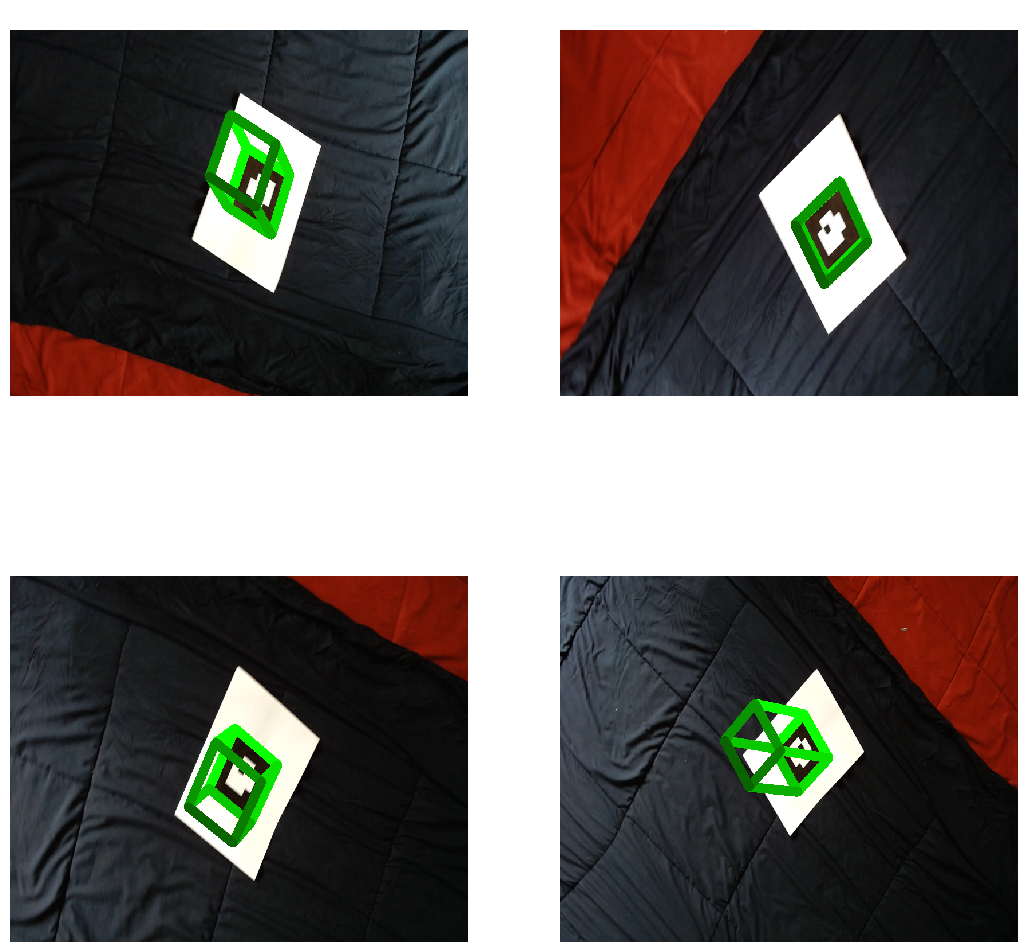
\includegraphics[width=\columnwidth]{/Q2/AR_Cube_Projection.png}
			\caption{Projecting the AR Cube}
			\label{fig:ARCube}
		\end{figure}
		
	
		
		\section{Extra Credit}
		
		Two types of Edge detection are performed on the Cityscape image show in Figure: \ref{fig:cityscape}. The first method is by using Canny edge detection and the second is by using DexiNed. DexiNed(Dense EXtreme Inception Network for Edge Detection) is a CNN based Edge detector.
		
		Contrasting with many CNN type architectures, all of them has a feature extraction backbone that fed their multi-layer feature outputs to
		corresponding upsampling layers, while DexiNed used a more robust Dense Extreme Inception architecture with residual style skip connections to extract and	propagate far richer edge feature information to deeper layers in the network.
		
		• They all use an upsampling layer to reproduce scaled intermediate edge maps at different
		layers within the network. The multi-level intermediate maps are then fused together to
		create a final output.
		
		• DexiNed uses depthwise separable convolutions and extracts more edge feature information which is learned in deeper layers of the network.
		
		• The accuracy of the results of each model was also mainly impacted by how robust it’s
		feature extraction backbone was. DexiNed which used a dense extreme inception network
		performed better than neural networks with backbone architectures such as ResNet-50 and VGG-16. From this observation, it is concluded that using a robust feature extractor is crucial
		in producing accurate edge maps.
		
		• In summary, the above-listed edge detection architecture share similar traits. They have a rich feature extractors and finally upscaled near the output layer.
		
		\begin{figure}[H]
			\centering
			\includegraphics[width=\columnwidth]{/cityscape1.png}
			\caption{Canny Edge detection}
			\label{fig:cityscape}
		\end{figure}
		
		
		\begin{figure}[H]
			\centering
			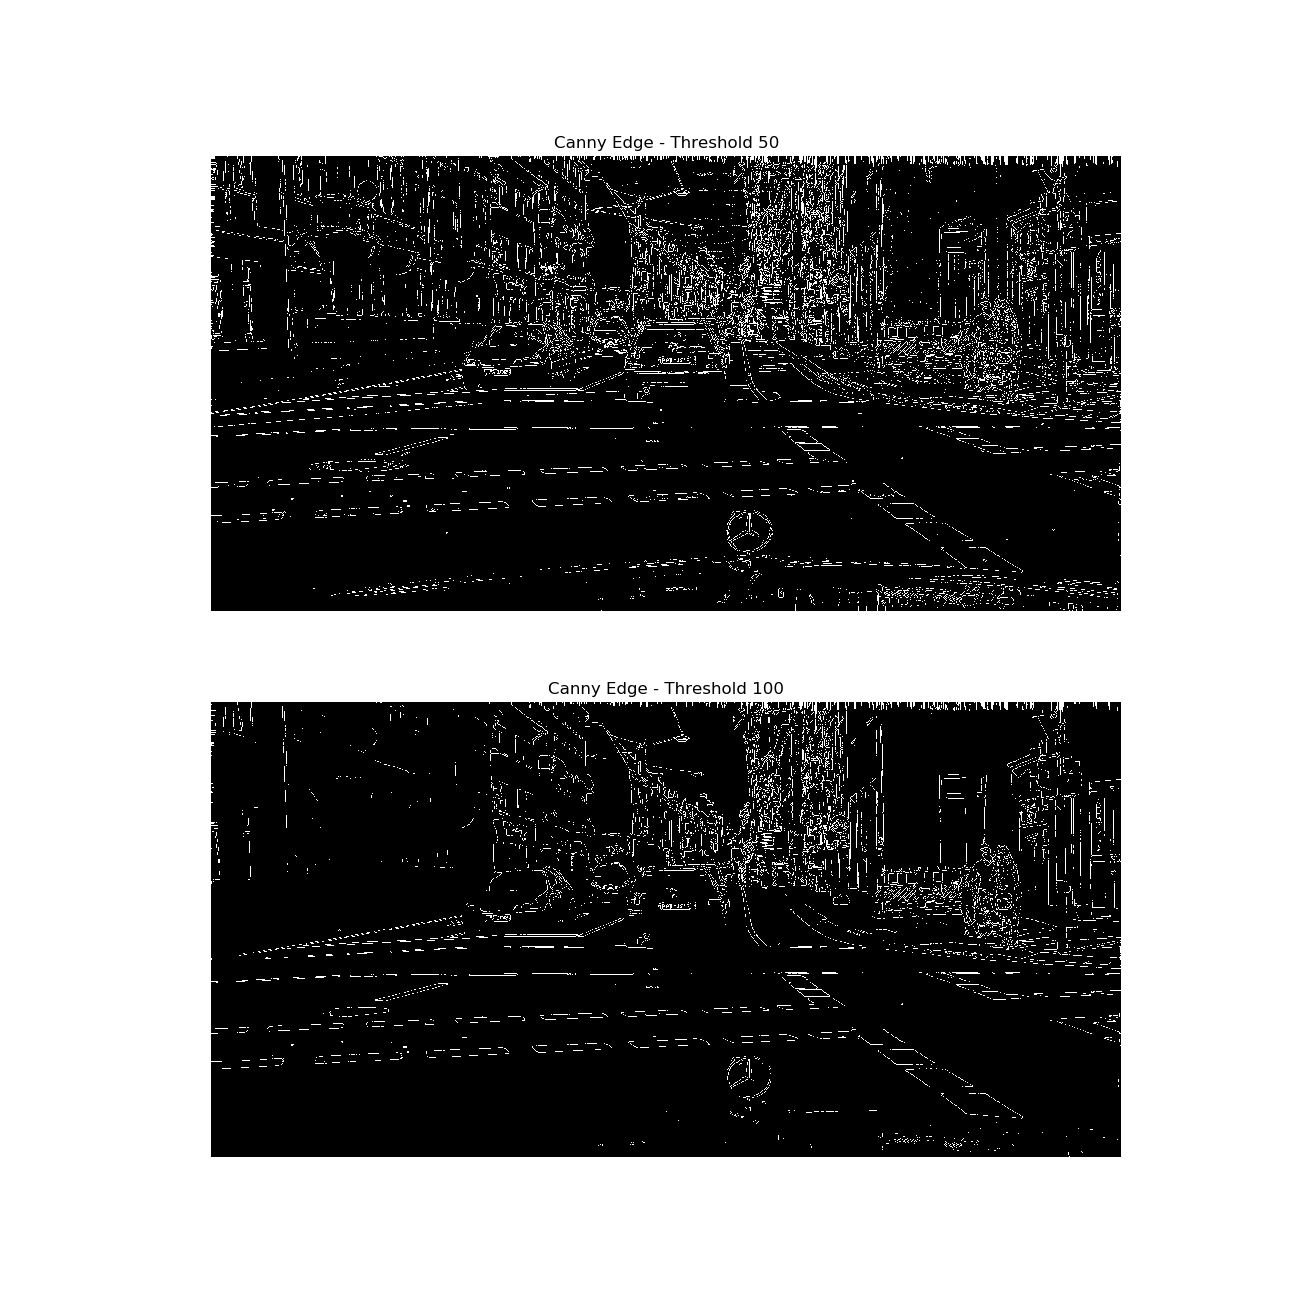
\includegraphics[width=\columnwidth]{/ExtraCredit/CannyEdge.png}
			\caption{Canny Edge detection}
			\label{fig:Canny}
		\end{figure}
		
		\begin{figure}[H]
			\centering
			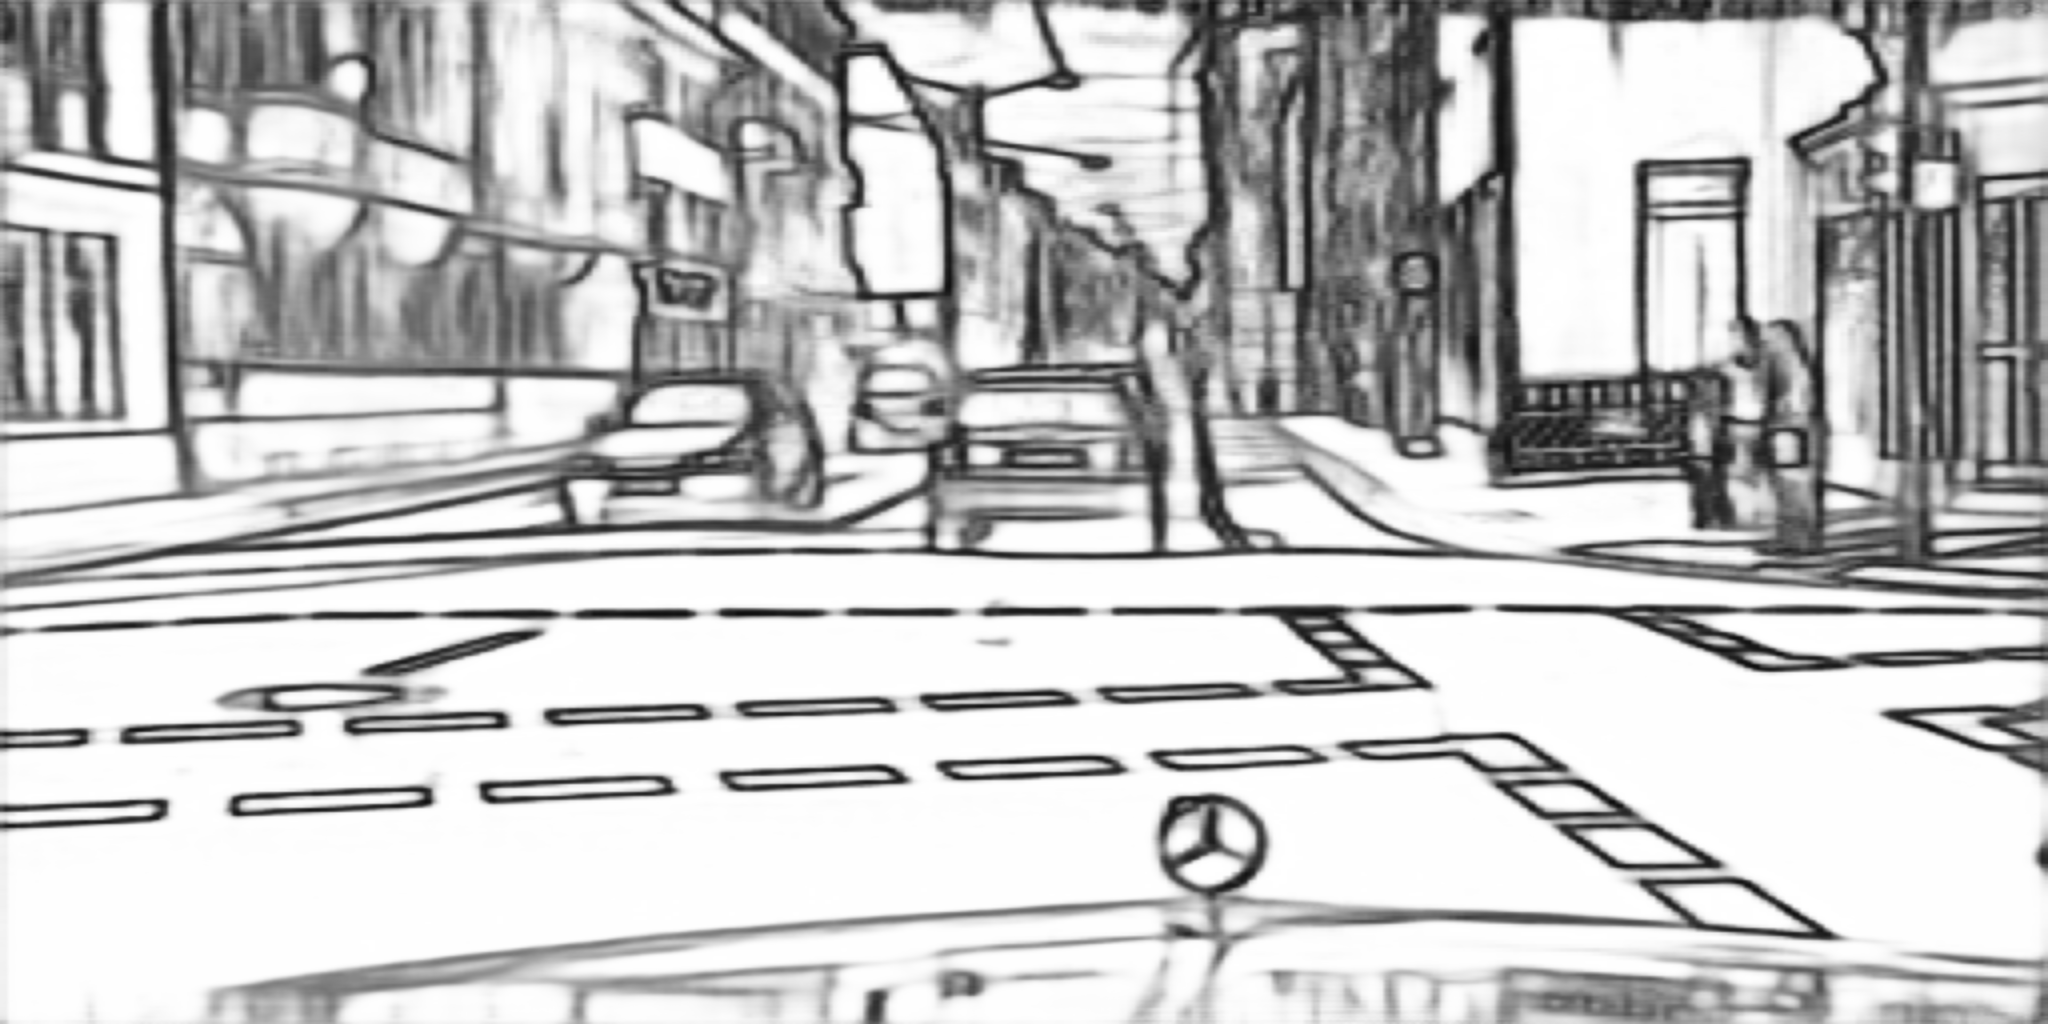
\includegraphics[width=\columnwidth]{/ExtraCredit/cityscape_avg.png}
			\caption{Edge Detection with DexiNed}
			\label{fig:DexiNed}
		\end{figure}
		
		
	\end{multicols}
	
\end{document}
